%--------------------------------------------------
\section{Sea level in context}

Sea level plays a unique role in physical oceanography. A role at least partly be attributed to it's \emph{observability}\citep{Wilson:2010hy}.


The present study will be limited to forecasts of sea level over time scales of hours to days; variations that basically constitute `the tides' as far as the general public is concerned.

\begin{figure}[h]\centering
  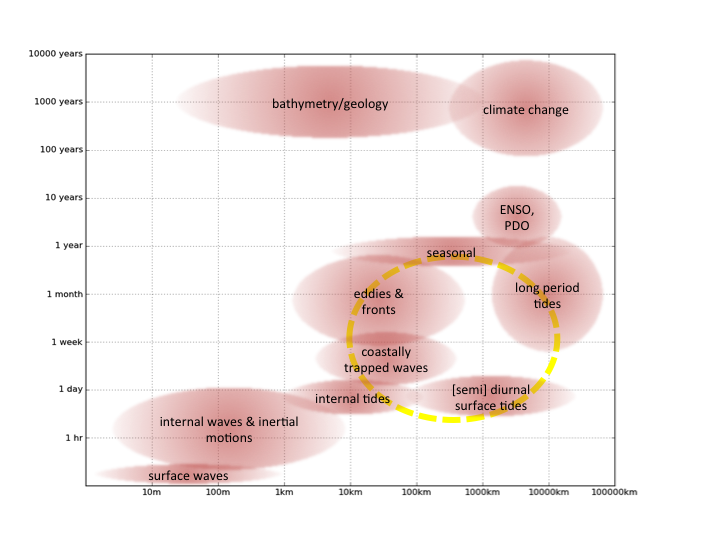
\includegraphics[width=130mm]{figures/diagrams/ocean_scales.png}
  \caption{Schematic indication of time/length scales of ocean processes.  The approximate scale limits for this research are highlighted. (Following \citet{Chelton:2001ws} )}
  \label{fig:SCALES}
\end{figure}

\begin{figure}[h]\centering
  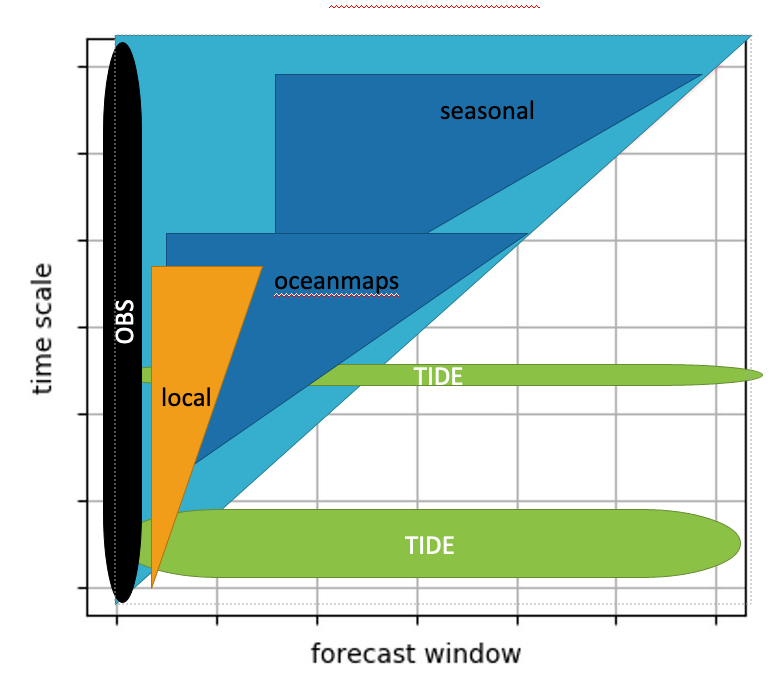
\includegraphics[width=80mm]{figures/images/sealevel_cartoon.png}
  \caption{Simplified illustration of the relative nature of sea level and different observing platforms.}
  \label{fig:SEALEVEL}
\end{figure}


\begin{figure}[h]\centering
	\subfloat[Darwin in Northern Australia - large diurnal tide.]{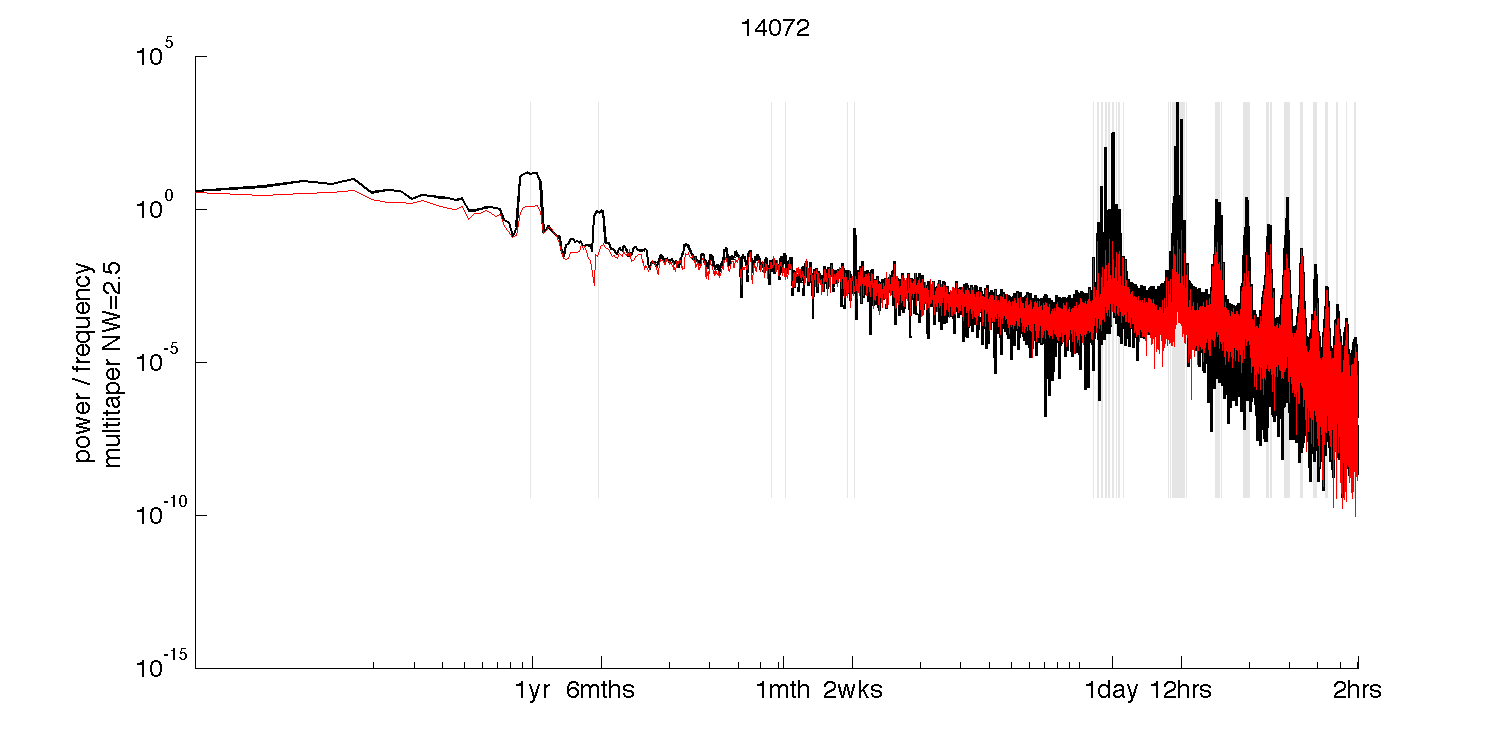
\includegraphics[width=130mm]{figures/images/plot_14072.png}} \\
	\subfloat[Esperence in Southern Australia - powerful synoptic signal.]{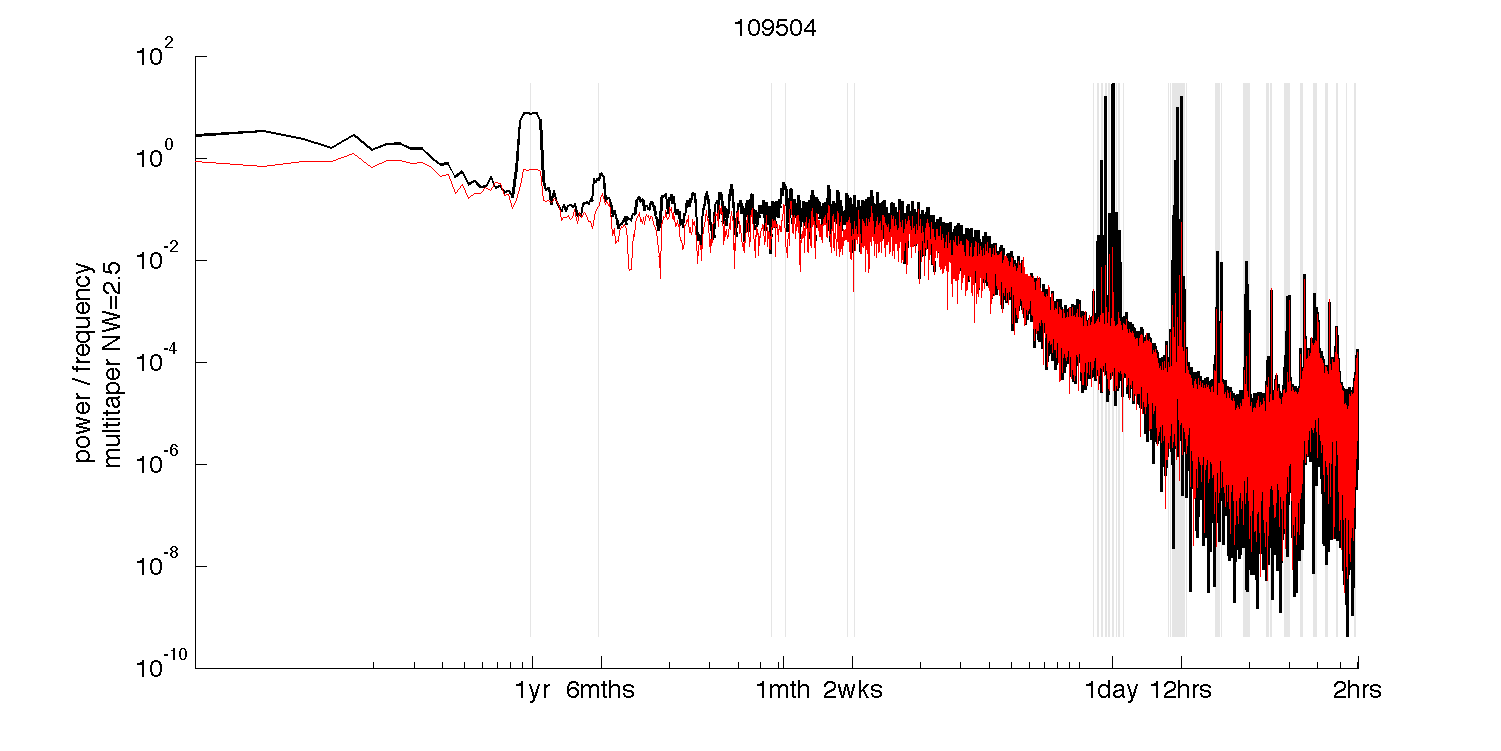
\includegraphics[width=130mm]{figures/images/plot_109504.png}}
	\caption{Spectral estimates from two coastal tide gauges. Hourly data, black = observations, red = tidal residual. An example of a `mixed spectra' \citep{Percival:1998tw}, in the sense of that discrete spectral lines appear embedded in a background continuum of coloured noise.  The overall `redness' of the spectra and the prominence of spikes at tidal frequencies is highlighted }
    \label{fig:SPECTRA_EG}
\end{figure}


%--------------------------------------------------
\subsection{Operational forecast setting}
\label{S:operational_setting}

Operational considerations are relevant to this review, which does not launch neatly from a single `conversation' \citep{Booth:2009vy} in the scientific literature.\\
Unfortunately operational documentation often falls far behind aspirations.
Tidal observation manuals exist eg \citep{IOC:2005tj}, \citep{Level:2011wu}, \citep{Parker:2007wq}.  However, analysis methods and design justifications are less formally documented - if at all.  The IOC understates this situation simply: `many organizations have developed their own method of tidal analysis'\citep{IOC:2005tj}\\

User expectations of sea level forecasts have largely been defined by harmonic tidal prediction practice. 
Conversely operational practice have influenced oceanography more broadly. Doodson's \citep{Doodson:1928wf} tidal procedures reflect the practical limits imposed by human computers and paper records, but have ongoing influence. \\


%--------------------------------------------------
\subsection{Future directions for forecast development}

BoM research strategy.


More general:

\begin{itemize}
  \item Towards 'concrete' , increasingly realistic and inclusive primitive equation forward models.
Peterson M1 ]\citep{Petersen:2012tr}
 \item Towards data-driven, service target - idealised, simple and robust 
\end{itemize}

%-------------------------------------------------- 
\subsection{Intersection of prediction perspectives}
\label{S:two_perspectives}

Tidal harmonic methods have for many decades provided the only routine source of sea level forecast - and with great success.  
In contrast, time stepping primitive equation dynamic models and data assimilation are relatively new arrivals to operational centres.  
These represent two qualitatively different perspectives on sea level prediction.\\


Over the past decade, the operational evolution of \OGCM-based prediction has increasingly brought the two approaches into something akin to Gallison's `trading zone' \citep{Galison:1996uc}.
Developments promise only to increase the amount of overlap into the previously independent practices of harmonic analysis, eg \cite{Arbic:2010us}.\\
Here Munk and Cartwright's aphorism from the 1960's regarding tidal analysis is illustrative:
\begin{quote}
  \dots predicting and learning are in a sense orthogonal, and the most interesting effects are those that cause the most trouble with a forecasting: the continuum, the nongravitational tides, and the non-linear interactions.\citep{Munk:1966ts} 
\end{quote}
Forecasts from \BL{} and other similar systems now represent sea level attributable to exactly these troublesome areas; or at least some physical subset therein.
Jayne's reference to the ``vexing problems'' \citep[pp812]{Jayne:2001tr} arising from applying frequency-domain theory in time-domain numerical tide modelling is illustrative.

\begin{figure}[h]\centering
  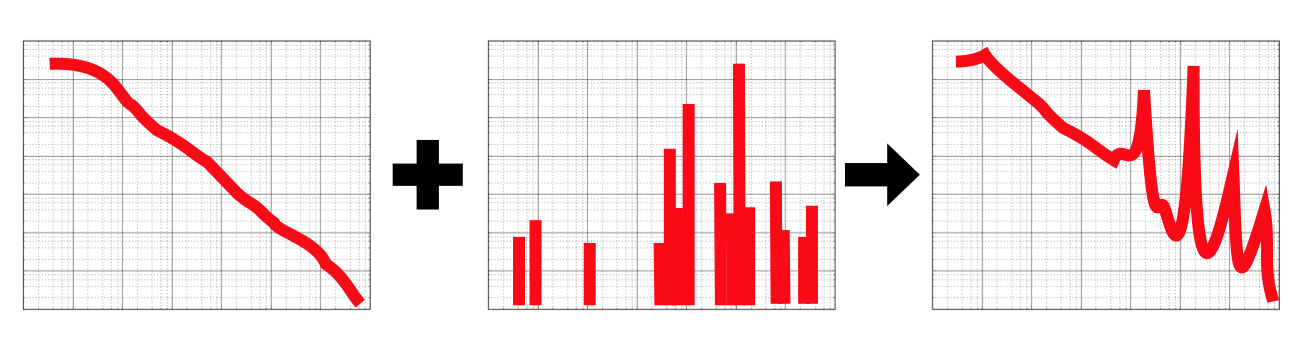
\includegraphics[width=120mm]{figures/diagrams/spectra_cartoon_1.png}
  \caption{Conventional decomposition concept: mixed sea level spectra comprising discrete tidal `lines' and red turbulent continuum.  Implementation of this concept has ramifications for sea level forecasting.}
  \label{fig:SPECTRA_CARTOON}
\end{figure}

Viewing sea level as a stationary set of harmonics is at face value quite at odds with a view of the ocean as a turbulent fluid.   In that sense, Gallison's portrayal of physics as `neither unified nor splintered into isolated fragments' \citep[pp 782]{Galison:1987wh} is apt.  Thus also is Peterson's assertion of `\dots{} the fundamental plurality of \dots{} scientific practice' \cite{Petersen:2012tr}. 
